\documentclass[14pt]{extarticle}
\usepackage{fontspec}
\usepackage{polyglossia}
\usepackage{amsmath}
\usepackage{amssymb}
\usepackage{xcolor}
\usepackage{fancyhdr}
\usepackage{graphicx}
\usepackage{listings}
\usepackage[most]{tcolorbox}
% \usepackage{setspace}
\usepackage{pifont}
\usepackage{enumitem}
\usepackage{titlesec}
\usepackage[bottom]{footmisc}
\usepackage{titling}
\usepackage{minted}
\usepackage{etoolbox}
\usepackage{array}
\usepackage{extsizes}
\usepackage{float}
\usepackage{booktabs}
\usepackage{hyperref}
\usepackage[onehalfspacing]{setspace}
\usepackage[a4paper, top=2.7cm, bottom=2.7cm, left=2.5cm, right=2.5cm, headheight=1.5cm, headsep=0.5cm]{geometry}
\usepackage{tikz}

\usetikzlibrary{automata, positioning, arrows.meta, arrows}

\newfontfamily\emoji{Segoe UI Emoji}

\pagestyle{fancy}

\setmainlanguage[numerals=western]{arabic}
\setotherlanguage{english}
% \newfontfamily\arabicfont[Script=Arabic]{Amiri}
\newfontfamily\arabicfont[Script=Arabic]{Calibri}
\newfontfamily\arabicfonttt[Script=Arabic]{Courier New}

\lstset{
  language=[Sharp]C,
  numbers=left,
  stepnumber=1,
  numbersep=8pt,
  frame=single,
  basicstyle=\ttfamily\small,
  keywordstyle=\color{blue},
  stringstyle=\color{red},
  commentstyle=\color{green!50!black}
}

\newif\ifdetailed
\ifdefined\setdetailed
  \setdetailed
\fi

\newif\ifwithsols
\ifdefined\setwithsols
  \setwithsols
\fi

% unified tcolorboxes for articles
\tcbset{colback=white, colframe=black, fonttitle=\bfseries, boxrule=0.8pt}
\newtcolorbox{boxDef}[1][]{colback=blue!5!white,colframe=blue!75!black,
  title={{\emoji📘} تعريف\ifx\\#1\\\else ~#1\fi :}}
\newtcolorbox{boxExercise}[1][]{colback=cyan!5!white,colframe=cyan!70!black,
  title={{\emoji🧩} تمرين\ifx\\#1\\\else ~#1\fi :}}
\newtcolorbox{boxExample}[1][]{colback=yellow!5!white,colframe=orange!90!black,
  title={{\emoji📝} مثال\ifx\\#1\\\else ~#1\fi :}}
\newtcolorbox{boxNote}[1][]{colback=gray!10!white,colframe=black,
  title={{\emoji✨} ملاحظة\ifx\\#1\\\else ~#1\fi :}}
\newtcolorbox{boxAttention}[1][]{colback=magenta!10!white,colframe=magenta!80!black,
  title={{\emoji🔔} تنبيه\ifx\\#1\\\else ~#1\fi :}}
\newtcolorbox{boxWarning}[1][]{colback=red!5!white,colframe=red!75!black,
  title={{\emoji⚡} ملاحظة هامة\ifx\\#1\\\else ~#1\fi :}}
\newtcolorbox{boxSolution}[1][]{colback=green!5!white,colframe=green!60!black,
  title={{\emoji✅} حل\ifx\\#1\\\else ~#1\fi :}}
\newtcolorbox{boxSymbol}[1][]{colback=purple!5!white,colframe=purple!70!black,
  title={{\emoji🔣} رمز\ifx\\#1\\\else ~#1\fi :}}
\newtcolorbox{boxHint}[1][]{colback=teal!5!white,colframe=teal!60!black,
  title={{\emoji💡} تلميح\ifx\\#1\\\else ~#1\fi :}}


\tcbset{simplecode/.style={ colback=gray!5, colframe=black!50, boxrule=0.4pt, arc=2pt, left=4pt,right=4pt,top=4pt,bottom=4pt}}
\newenvironment{boxCode}{\begin{tcolorbox}[simplecode]}{\end{tcolorbox}}

\newcolumntype{C}[1]{>{\centering\arraybackslash}p{#1}}

% redefine spaces after titles
\makeatletter
\renewcommand{\@maketitle}{%
  \begin{center}
    {\huge \bfseries \@title \par}%
    \vskip 0.2em % space between title and author
    {\large \@author \par}%
    % \vskip 0.2em % space between author and date
    % {\normalsize \@date \par}%
  \end{center}
}
\makeatother

\fancyhf{} % clear default
\fancypagestyle{plain}{
  \fancyhf{}
  \fancyhead[L]{مدرسة التسامح الشاملة}
  % \fancyhead[L]{
\includegraphics[height=1cm]{../../../images/logoTasamoh.png}}
  \fancyhead[R]{الأستاذ محمود اغبارية}
  \fancyfoot[C]{\thepage}
}

\fancyhead[L]{مدرسة التسامح الشاملة}
\fancyhead[R]{الأستاذ محمود اغبارية}
\fancyfoot[C]{\thepage}
% \date{\today}

\setcounter{tocdepth}{3} % only section subsection and subsubsection in TOC

\newcommand{\importpdfpage}[2]{%
    \thispagestyle{empty}
    \newgeometry{left=0cm,right=0cm,top=0cm,bottom=0cm}
    \includegraphics[page=#2,width=0.95\paperwidth,height=0.95\paperheight,keepaspectratio]{#1}
    \restoregeometry
}

\newcommand{\insertFullImg}[1]{%
    \noindent
    \makebox[\textwidth][c]{
        \includegraphics[width=0.9\paperwidth,keepaspectratio]{#1}%
    }%
}%

% ----------------------


% \begin{document}

% \maketitle

% % \clearpage  % start TOC on a new page
% % \renewcommand{\contentsname}{جدول المحتويات}
% % \tableofcontents
% % \clearpage

% \part*{part 1} % the * prevents numbering
% \section*{مقدمة}
% \subsection*{مثال رياضي}
% \subsubsection*{مثال فرعي}
% \paragraph*{ paragraph 1}
% \subparagraph*{sub paragraph 1}

% \ifdetailed
% \begin{english}
% \begin{minted}{csharp}
% // C# Example
% \end{minted}
% \end{english}
% \fi

% OLD WAY
% \ifdetailed
% \begin{english}
% \begin{lstlisting}
% // C# Example
% \end{lstlisting}
% \end{english}
% \fi

% % 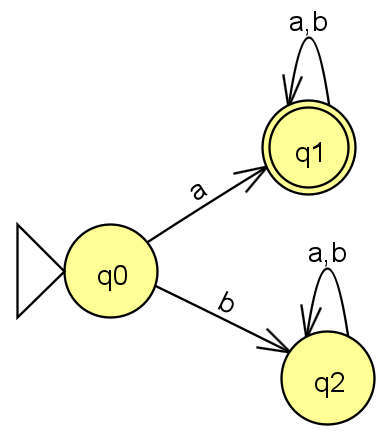
\includegraphics[width=0.2\textwidth]{../../../images/DFAs/ex1_q1.png}



% \vspace{3cm}
% \begin{flushleft}
% أرجو لكم وقتًا ممتعًا.

% الأستاذ محمود اغبارية.
% \end{flushleft}


% \end{document}


\ifwithsols
\title{حل - المصفوفات الأحادية - مجموعة شاملة منظمة}
\else
\title{المصفوفات الأحادية - مجموعة شاملة منظمة}
\fi

\begin{document}

\maketitle
\thispagestyle{fancy}

\tableofcontents
\clearpage

% =====================================================
% القسم 1: أسئلة تأسيسية
% =====================================================
\section{أسئلة تأسيسية}

\begin{enumerate}[itemsep=2em]

    % ======================================================
    % 1. التصريح والتهيئة الأساسية
    % ======================================================
    \item
    أ) صرح عن مصفوفة أعداد صحيحة (\textenglish{int}) باسم \textenglish{numbers} تتسع لـ 10 عناصر.\\
    ب) صرح عن مصفوفة نصوص (\textenglish{string}) باسم \textenglish{colors} وامنحها القيم الأولية: \textenglish{"Red", "Green", "Blue"}.
    \ifwithsols
    \begin{boxSolution}
    \begin{english}
    \begin{minted}{csharp}
// A
int[] numbers = new int[10];

// B
string[] colors = { "Red", "Green", "Blue" };
    \end{minted}
    \end{english}
    \end{boxSolution}
    \fi

    % ======================================================
    % 2. ملء مصفوفة بقيمة ثابتة
    % ======================================================
    \item
    عرف مصفوفة أعداد صحيحة طولها 10، ثم اكتب حلقة تكرار لملء جميع خاناتها بالقيمة $-1$.
    \ifwithsols
    \begin{boxSolution}
    \begin{english}
    \begin{minted}{csharp}
int[] arr = new int[10];
for (int i = 0; i < arr.Length; i++)
{
    arr[i] = -1;
}
    \end{minted}
    \end{english}
    \end{boxSolution}
    \fi

    % ======================================================
    % 3. الوصول للعنصر الأول والأخير
    % ======================================================
    \item
    لديك مصفوفة أعداد صحيحة باسم \textenglish{data}. اكتب مقطع برنامج يطبع العنصر الأول والعنصر الأخير فيها. (افترض أن المصفوفة ليست فارغة).
    \ifwithsols
    \begin{boxSolution}
    \begin{english}
    \begin{minted}{csharp}
Console.WriteLine("First: " + data[0]);
Console.WriteLine("Last: " + data[data.Length - 1]);
    \end{minted}
    \end{english}
    \end{boxSolution}
    \fi

    % ======================================================
    % 4. طباعة بترتيب عكسي
    % ======================================================
    \item
    اكتب حلقة لطباعة عناصر مصفوفة النصوص \textenglish{names} بترتيب عكسي (من آخر عنصر إلى أول عنصر).\\
    \textbf{مثال:} إذا كانت المصفوفة \textenglish{\{"A", "B", "C"\}} يطبع البرنامج \textenglish{C} ثم \textenglish{B} ثم \textenglish{A}.
    \ifwithsols
    \begin{boxSolution}
    \begin{english}
    \begin{minted}{csharp}
for (int i = names.Length - 1; i >= 0; i--)
{
    Console.WriteLine(names[i]);
}
    \end{minted}
    \end{english}
    \end{boxSolution}
    \fi

    % ======================================================
    % 5. طباعة القيم الزوجية
    % ======================================================
    \item
    اكتب مقطع برنامج يطبع القيم الموجودة في الخانات الزوجية فقط (0, 2, 4...) لمصفوفة أعداد صحيحة \textenglish{arr}.
    \ifwithsols
    \begin{boxSolution}
    \begin{english}
    \begin{minted}{csharp}
for (int i = 0; i < arr.Length; i += 2)
{
    Console.WriteLine(arr[i]);
}
    \end{minted}
    \end{english}
    \end{boxSolution}
    \fi

    % ======================================================
    % 6. إضافة قيمة لكل عنصر
    % ======================================================
    \item
    لديك مصفوفة درجات طلاب \textenglish{scores} (أعداد صحيحة). اكتب مقطع برنامج يضيف 5 درجات لكل طالب في المصفوفة (تعديل القيم داخل نفس المصفوفة).
    \ifwithsols
    \begin{boxSolution}
    \begin{english}
    \begin{minted}{csharp}
for (int i = 0; i < scores.Length; i++)
{
    scores[i] += 5;
}
    \end{minted}
    \end{english}
    \end{boxSolution}
    \fi

    % ======================================================
    % 7. جمع مصفوفتين
    % ======================================================
    \item
    اكتب مقطع برنامج يجمع عناصر مصفوفتين من الأعداد الصحيحة \textenglish{A} و \textenglish{B} (لهما نفس الطول) ويخزن الناتج في مصفوفة جديدة \textenglish{C}.\\
    بحيث يكون: $C[i] = A[i] + B[i]$.
    \ifwithsols
    \begin{boxSolution}
    \begin{english}
    \begin{minted}{csharp}
int[] C = new int[A.Length];
for (int i = 0; i < A.Length; i++)
{
    C[i] = A[i] + B[i];
}
    \end{minted}
    \end{english}
    \end{boxSolution}
    \fi

    % ======================================================
    % 8. عد العناصر الموجبة
    % ======================================================
    \item
    اكتب مقطع برنامج يحسب عدد العناصر الموجبة في مصفوفة الأعداد الصحيحة \textenglish{numbers}.
    \ifwithsols
    \begin{boxSolution}
    \begin{english}
    \begin{minted}{csharp}
int count = 0;
for (int i = 0; i < numbers.Length; i++)
{
    if (numbers[i] > 0)
        count++;
}
Console.WriteLine("Positive count: " + count);
    \end{minted}
    \end{english}
    \end{boxSolution}
    \fi

    % ======================================================
    % 9. مجموع الخانات الفردية
    % ======================================================
    \item
    اكتب مقطع برنامج يحسب مجموع العناصر الموجودة في الخانات الفردية لمصفوفة أعداد صحيحة \textenglish{arr}.
    \ifwithsols
    \begin{boxSolution}
    \begin{english}
    \begin{minted}{csharp}
int sum = 0;
for (int i = 1; i < arr.Length; i += 2)
{
    sum += arr[i];
}
Console.WriteLine("Sum at odd indices: " + sum);
    \end{minted}
    \end{english}
    \end{boxSolution}
    \fi

    % ======================================================
    % 10. عد عناصر في مجال
    % ======================================================
    \item
    اكتب مقطع برنامج يعد كم عنصراً في مصفوفة العلامات \textenglish{grades} يقع ضمن المجال $[60, 80]$ (أي أكبر أو يساوي 60 وأصغر أو يساوي 80).
    \ifwithsols
    \begin{boxSolution}
    \begin{english}
    \begin{minted}{csharp}
int count = 0;
for (int i = 0; i < grades.Length; i++)
{
    if (grades[i] >= 60 && grades[i] <= 80)
        count++;
}
Console.WriteLine("Count in range [60-80]: " + count);
    \end{minted}
    \end{english}
    \end{boxSolution}
    \fi

    % ======================================================
    % 11. البحث عن أول عنصر سالب
    % ======================================================
    \item
    اكتب مقطع برنامج يبحث عن \textbf{أول} عدد سالب في مصفوفة أعداد صحيحة \textenglish{arr}.
    إذا وجده يطبع قيمته وموقعه ثم يتوقف عن البحث.
    \ifwithsols
    \begin{boxSolution}
    \begin{english}
    \begin{minted}{csharp}
for (int i = 0; i < arr.Length; i++)
{
    if (arr[i] < 0)
    {
        Console.WriteLine($"Found negative {arr[i]} at index {i}");
        break;
    }
}
    \end{minted}
    \end{english}
    \end{boxSolution}
    \fi

    % ======================================================
    % 12. فحص وجود قيمة
    % ======================================================
    \item
    اكتب مقطع برنامج يفحص هل العدد \textenglish{50} موجود داخل المصفوفة \textenglish{numbers} أم لا، ويطبع \textenglish{"Found"} أو \textenglish{"Not Found"}.
    \ifwithsols
    \begin{boxSolution}
    \begin{english}
    \begin{minted}{csharp}
bool found = false;
for (int i = 0; i < numbers.Length; i++)
{
    if (numbers[i] == 50)
    {
        found = true;
        break;
    }
}
if (found) Console.WriteLine("Found");
else Console.WriteLine("Not Found");
    \end{minted}
    \end{english}
    \end{boxSolution}
    \fi

    % ======================================================
    % 13. الفرق بين أكبر وأصغر قيمة
    % ======================================================
    \item
    اكتب مقطع برنامج يحسب ويطبع الفرق بين أكبر قيمة وأصغر قيمة في مصفوفة أعداد صحيحة \textenglish{data}.\\
    \textbf{مثال:} إذا كانت المصفوفة تحتوي على \textenglish{\{3, 10, 6, 1\}}، الفرق هو $10 - 1 = 9$.
    \ifwithsols
    \begin{boxSolution}
    \begin{english}
    \begin{minted}{csharp}
if (data.Length > 0) {
    int max = data[0];
    int min = data[0];
    for (int i = 1; i < data.Length; i++)
    {
        if (data[i] > max) max = data[i];
        if (data[i] < min) min = data[i];
    }
    Console.WriteLine("Difference: " + (max - min));
}
    \end{minted}
    \end{english}
    \end{boxSolution}
    \fi

    % ======================================================
    % 14. قراءة وطباعة أكبر من المعدل
    % ======================================================
    \item
    اكتب برنامجاً يقرأ 10 أعداد صحيحة من المستخدم ويطبع له كل الأعداد الأكبر من معدل الـ 10 أعداد كلها.\\
    \textbf{مثال:} إذا أدخل المستخدم الأعداد: 5, 10, 15, 20, 25, 30, 35, 40, 45, 50، يكون المعدل هو $27.5$، والأعداد الأكبر من المعدل هي: 30, 35, 40, 45, 50.
    \ifwithsols
    \begin{boxSolution}
    \begin{english}
    \begin{minted}{csharp}
int[] userNums = new int[10];
int sum = 0;

for (int i = 0; i < userNums.Length; i++)
{
    userNums[i] = int.Parse(Console.ReadLine());
    sum += userNums[i];
}

double avg = (double)sum / userNums.Length;

for (int i = 0; i < userNums.Length; i++)
{
    if(userNums[i] > avg)
        Console.WriteLine(userNums[i]);
}
    \end{minted}
    \end{english}
    \end{boxSolution}
    \fi

\end{enumerate}

\clearpage

% =====================================================
% القسم 2: أسئلة أساسية لمصفوفة مع عمليات خارجية
% =====================================================
\section{أسئلة أساسية - عمليات خارجية}

\begin{enumerate}[resume, itemsep=2em]

    % ======================================================
    % 15. GetMax
    % ======================================================
    \item
    اكتب عملية خارجية \textenglish{int GetMax(int[] arr)} تستقبل مصفوفة أعداد صحيحة وتعيد أكبر قيمة فيها.\\
    \textbf{مثال:} إذا كانت المصفوفة \textenglish{\{5, 12, 8, 20, 3\}}، تعيد العملية 20.
    \ifwithsols
    \begin{boxSolution}
    \begin{english}
    \begin{minted}{csharp}
public static int GetMax(int[] arr)
{
    int max = arr[0];
    for (int i = 1; i < arr.Length; i++)
    {
        if (arr[i] > max)
            max = arr[i];
    }
    return max;
}
    \end{minted}
    \end{english}
    \end{boxSolution}
    \fi

    % ======================================================
    % 16. GetMin
    % ======================================================
    \item
    اكتب عملية خارجية \textenglish{int GetMin(int[] arr)} تستقبل مصفوفة أعداد صحيحة وتعيد أصغر قيمة فيها.\\
    \textbf{مثال:} في المصفوفة \textenglish{\{15, 3, 9, 21, 7\}} أصغر قيمة هي 3.
    \ifwithsols
    \begin{boxSolution}
    \begin{english}
    \begin{minted}{csharp}
public static int GetMin(int[] arr)
{
    int min = arr[0];
    for (int i = 1; i < arr.Length; i++)
    {
        if (arr[i] < min)
            min = arr[i];
    }
    return min;
}
    \end{minted}
    \end{english}
    \end{boxSolution}
    \fi

    % ======================================================
    % 17. GetAverage
    % ======================================================
    \item
    اكتب عملية خارجية \textenglish{double GetAverage(int[] arr)} تستقبل مصفوفة أعداد صحيحة وتعيد معدل جميع عناصرها.\\
    \textbf{مثال:} في المصفوفة \textenglish{\{10, 20, 30, 40\}} المعدل هو $\frac{10+20+30+40}{4} = 25.0$
    \ifwithsols
    \begin{boxSolution}
    \begin{english}
    \begin{minted}{csharp}
public static double GetAverage(int[] arr)
{
    int sum = 0;
    for (int i = 0; i < arr.Length; i++)
    {
        sum += arr[i];
    }
    return (double)sum / arr.Length;
}
    \end{minted}
    \end{english}
    \end{boxSolution}
    \fi

    % ======================================================
    % 18. CountNegative
    % ======================================================
    \item
    اكتب عملية خارجية \textenglish{int CountNegative(int[] arr)} تستقبل مصفوفة أعداد صحيحة وتعيد عدد الأعداد السالبة فيها.\\
    \textbf{مثال:} في المصفوفة \textenglish{\{5, -3, 8, -7, 0, -1\}} يوجد 3 أعداد سالبة.
    \ifwithsols
    \begin{boxSolution}
    \begin{english}
    \begin{minted}{csharp}
public static int CountNegative(int[] arr)
{
    int count = 0;
    for (int i = 0; i < arr.Length; i++)
    {
        if (arr[i] < 0)
            count++;
    }
    return count;
}
    \end{minted}
    \end{english}
    \end{boxSolution}
    \fi

    % ======================================================
    % 19. CountEven
    % ======================================================
    \item
    اكتب عملية خارجية \textenglish{int CountEven(int[] arr)} تستقبل مصفوفة أعداد صحيحة وتعيد عدد الأعداد الزوجية فيها.\\
    \textbf{مثال:} في المصفوفة \textenglish{\{5, 12, 7, 8, 3, 10\}} يوجد 3 أعداد زوجية (12, 8, 10).
    \ifwithsols
    \begin{boxSolution}
    \begin{english}
    \begin{minted}{csharp}
public static int CountEven(int[] arr)
{
    int count = 0;
    for (int i = 0; i < arr.Length; i++)
    {
        if (arr[i] % 2 == 0)
            count++;
    }
    return count;
}
    \end{minted}
    \end{english}
    \end{boxSolution}
    \fi

    % ======================================================
    % 20. SumPositive
    % ======================================================
    \item
    اكتب عملية خارجية \textenglish{int SumPositive(int[] arr)} تستقبل مصفوفة أعداد صحيحة وتعيد مجموع الأعداد الموجبة فقط (الأكبر من صفر).\\
    \textbf{مثال:} إذا تلقت المصفوفة \textenglish{\{5, -3, 8, -2, 0, 10\}}، تعيد $5 + 8 + 10 = 23$.
    \ifwithsols
    \begin{boxSolution}
    \begin{english}
    \begin{minted}{csharp}
public static int SumPositive(int[] arr)
{
    int sum = 0;
    for (int i = 0; i < arr.Length; i++)
    {
        if (arr[i] > 0)
            sum += arr[i];
    }
    return sum;
}
    \end{minted}
    \end{english}
    \end{boxSolution}
    \fi

    % ======================================================
    % 21. CountOccurrences
    % ======================================================
    \item
    اكتب عملية خارجية \textenglish{int CountOccurrences(int[] arr, int value)} تستقبل مصفوفة أعداد صحيحة وعدداً صحيحاً، وتعيد عدد مرات ظهور العدد في المصفوفة.\\
    \textbf{مثال:} في المصفوفة \textenglish{\{5, 12, 8, 12, 3, 12\}}، العدد 12 يظهر 3 مرات.
    \ifwithsols
    \begin{boxSolution}
    \begin{english}
    \begin{minted}{csharp}
public static int CountOccurrences(int[] arr, int value)
{
    int count = 0;
    for (int i = 0; i < arr.Length; i++)
    {
        if (arr[i] == value)
            count++;
    }
    return count;
}
    \end{minted}
    \end{english}
    \end{boxSolution}
    \fi

    % ======================================================
    % 22. Contains
    % ======================================================
    \item
    اكتب عملية خارجية \textenglish{bool Contains(int[] arr, int value)} تستقبل مصفوفة أعداد صحيحة وعدداً صحيحاً، وتعيد \textenglish{true} إذا كان العدد موجوداً في المصفوفة، وإلا تعيد \textenglish{false}.\\
    \textbf{مثال:}
    \begin{itemize}
        \item \textenglish{Contains(\{5, 10, 15, 20\}, 15)} $\leftarrow$ \textenglish{true}
        \item \textenglish{Contains(\{5, 10, 15, 20\}, 7)} $\leftarrow$ \textenglish{false}
    \end{itemize}
    \ifwithsols
    \begin{boxSolution}
    \begin{english}
    \begin{minted}{csharp}
public static bool Contains(int[] arr, int value)
{
    for (int i = 0; i < arr.Length; i++)
    {
        if (arr[i] == value)
            return true;
    }
    return false;
}
    \end{minted}
    \end{english}
    \end{boxSolution}
    \fi

    % ======================================================
    % 23. FindIndex
    % ======================================================
    \item
    اكتب عملية خارجية \textenglish{int FindIndex(int[] arr, int val)} تعيد رقم الخانة (Index) لأول ظهور للقيمة \textenglish{val} في المصفوفة. إذا لم تجدها تعيد $-1$.\\
    \textbf{مثال:} إذا كانت المصفوفة \textenglish{\{10, 20, 30, 40\}}:
    \begin{itemize}
        \item \textenglish{FindIndex(arr, 30)} تعيد 2
        \item \textenglish{FindIndex(arr, 50)} تعيد $-1$
    \end{itemize}
    \ifwithsols
    \begin{boxSolution}
    \begin{english}
    \begin{minted}{csharp}
public static int FindIndex(int[] arr, int val)
{
    for (int i = 0; i < arr.Length; i++)
    {
        if (arr[i] == val)
            return i;
    }
    return -1;
}
    \end{minted}
    \end{english}
    \end{boxSolution}
    \fi

    % ======================================================
    % 24. AreArraysEqual
    % ======================================================
    \item
    اكتب عملية خارجية \textenglish{bool AreArraysEqual(int[] arr1, int[] arr2)} تستقبل مصفوفتين من الأعداد الصحيحة وتعيد \textenglish{true} إذا كانتا متساويتين (نفس الطول ونفس العناصر بنفس الترتيب)، وإلا تعيد \textenglish{false}.\\
    \textbf{مثال:}
    \begin{itemize}
        \item \textenglish{\{1, 2, 3\}} و \textenglish{\{1, 2, 3\}} $\leftarrow$ \textenglish{true}
        \item \textenglish{\{1, 2, 3\}} و \textenglish{\{1, 2, 4\}} $\leftarrow$ \textenglish{false}
    \end{itemize}
    \ifwithsols
    \begin{boxSolution}
    \begin{english}
    \begin{minted}{csharp}
public static bool AreArraysEqual(int[] arr1, int[] arr2)
{
    if (arr1.Length != arr2.Length)
        return false;

    for (int i = 0; i < arr1.Length; i++)
    {
        if (arr1[i] != arr2[i])
            return false;
    }

    return true;
}
    \end{minted}
    \end{english}
    \end{boxSolution}
    \fi

    % ======================================================
    % 25. ReplaceNegativeWithZero
    % ======================================================
    \item
    اكتب عملية خارجية \textenglish{void ReplaceNegativeWithZero(int[] arr)} تستقبل مصفوفة أعداد صحيحة وتعدلها بحيث تستبدل كل عدد سالب فيها بالصفر.\\
    \textbf{مثال:} إذا كانت المصفوفة \textenglish{\{5, -3, 0, -7, 2\}}، تصبح بعد استدعاء العملية \textenglish{\{5, 0, 0, 0, 2\}}.
    \ifwithsols
    \begin{boxSolution}
    \begin{english}
    \begin{minted}{csharp}
public static void ReplaceNegativeWithZero(int[] arr)
{
    for (int i = 0; i < arr.Length; i++)
    {
        if (arr[i] < 0)
            arr[i] = 0;
    }
}
    \end{minted}
    \end{english}
    \end{boxSolution}
    \fi

    % ======================================================
    % 26. SumInRange
    % ======================================================
    \item
    اكتب عملية خارجية \textenglish{int SumInRange(int[] arr, int min, int max)} تستقبل مصفوفة أعداد صحيحة وقيمتين (\textenglish{min} و\textenglish{max})، وتعيد مجموع جميع الأعداد الواقعة ضمن المجال $[min, max]$ (شامل الطرفين).\\
    \textbf{مثال:} في المصفوفة \textenglish{\{5, 15, 25, 8, 30, 12, 3\}} مع \textenglish{min = 10} و\textenglish{max = 20}:
    \begin{itemize}
        \item الأعداد في المجال: 15، 12
        \item المجموع: $15 + 12 = 27$
    \end{itemize}
    \ifwithsols
    \begin{boxSolution}
    \begin{english}
    \begin{minted}{csharp}
public static int SumInRange(int[] arr, int min, int max)
{
    int sum = 0;
    for (int i = 0; i < arr.Length; i++)
    {
        if (arr[i] >= min && arr[i] <= max)
            sum += arr[i];
    }
    return sum;
}
    \end{minted}
    \end{english}
    \end{boxSolution}
    \fi

    % ======================================================
    % 27. GetMultiples
    % ======================================================
    \item
    اكتب عملية خارجية \textenglish{int[] GetMultiples(int[] arr, int factor)} تستقبل مصفوفة أعداد صحيحة وعدداً صحيحاً (\textenglish{factor})، وتعيد مصفوفة جديدة تحتوي فقط على الأعداد القابلة للقسمة على \textenglish{factor}.\\
    \textbf{مثال:} في المصفوفة \textenglish{\{12, 15, 18, 22, 24\}} مع \textenglish{factor = 3}:
    \begin{itemize}
        \item العناصر القابلة للقسمة: 12، 15، 18، 24
        \item النتيجة: \textenglish{\{12, 15, 18, 24\}}
    \end{itemize}
    \ifwithsols
    \begin{boxSolution}
    \begin{english}
    \begin{minted}{csharp}
public static int[] GetMultiples(int[] arr, int factor)
{
    int count = 0;
    for (int i = 0; i < arr.Length; i++)
    {
        if (arr[i] % factor == 0)
            count++;
    }

    int[] result = new int[count];
    int index = 0;
    for (int i = 0; i < arr.Length; i++)
    {
        if (arr[i] % factor == 0)
        {
            result[index] = arr[i];
            index++;
        }
    }

    return result;
}
    \end{minted}
    \end{english}
    \end{boxSolution}
    \fi

    % ======================================================
    % 28. FirstAboveAverage
    % ======================================================
    \item
    اكتب عملية خارجية \textenglish{int FirstAboveAverage(int[] arr)} تستقبل مصفوفة أعداد صحيحة وتعيد موقع (index) أول عنصر أكبر من معدل المصفوفة. إذا لم يوجد عنصر أكبر من المعدل، تعيد $-1$.\\
    \textbf{مثال:} في المصفوفة \textenglish{\{10, 5, 20, 15, 8\}}:
    \begin{itemize}
        \item المعدل = $\frac{10+5+20+15+8}{5} = 11.6$
        \item أول عنصر أكبر من المعدل هو 20 في الموقع 2
        \item النتيجة: 2
    \end{itemize}
    \ifwithsols
    \begin{boxSolution}
    \begin{english}
    \begin{minted}{csharp}
public static int FirstAboveAverage(int[] arr)
{
    int sum = 0;
    for (int i = 0; i < arr.Length; i++)
    {
        sum += arr[i];
    }

    double avg = (double)sum / arr.Length;

    for (int i = 0; i < arr.Length; i++)
    {
        if (arr[i] > avg)
            return i;
    }

    return -1;
}
    \end{minted}
    \end{english}
    \end{boxSolution}
    \fi

\end{enumerate}

\clearpage

% =====================================================
% القسم 3: أسئلة عكس المصفوفة
% =====================================================
\section{أسئلة عكس المصفوفة}

\begin{enumerate}[resume, itemsep=2em]

    % ======================================================
    % 29. تبديل أول وأخير
    % ======================================================
    \item
    اكتب عملية خارجية \textenglish{void SwapFirstLast(int[] arr)} تبدّل العنصر الأول مع العنصر الأخير في المصفوفة.\\
    \textbf{مثال:} إذا كانت المصفوفة \textenglish{\{5, 10, 15, 20\}}، تصبح بعد استدعاء العملية \textenglish{\{20, 10, 15, 5\}}.
    \ifwithsols
    \begin{boxSolution}
    \begin{english}
    \begin{minted}{csharp}
public static void SwapFirstLast(int[] arr)
{
    int temp = arr[0];
    arr[0] = arr[arr.Length - 1];
    arr[arr.Length - 1] = temp;
}
    \end{minted}
    \end{english}
    \end{boxSolution}
    \fi

    % ======================================================
    % 30. طباعة عكسية
    % ======================================================
    \item
    اكتب عملية خارجية \textenglish{void PrintReverse(int[] arr)} تطبع عناصر المصفوفة بترتيب عكسي (من الأخير إلى الأول)، كل عنصر في سطر منفصل.\\
    \textbf{مثال:} إذا كانت المصفوفة \textenglish{\{10, 20, 30\}}، تطبع:
    \begin{english}
    \begin{verbatim}
30
20
10
    \end{verbatim}
    \end{english}
    \ifwithsols
    \begin{boxSolution}
    \begin{english}
    \begin{minted}{csharp}
public static void PrintReverse(int[] arr)
{
    for (int i = arr.Length - 1; i >= 0; i--)
    {
        Console.WriteLine(arr[i]);
    }
}
    \end{minted}
    \end{english}
    \end{boxSolution}
    \fi

    % ======================================================
    % 31. نسخ بترتيب عكسي
    % ======================================================
    \item
    اكتب عملية خارجية \textenglish{int[] CopyReverse(int[] source)} تستقبل مصفوفة وتعيد مصفوفة جديدة تحتوي على نفس العناصر لكن بترتيب عكسي.\\
    \textbf{مثال:} إذا كانت \textenglish{source = \{10, 20, 30, 40\}}، تعيد \textenglish{\{40, 30, 20, 10\}}.
    \ifwithsols
    \begin{boxSolution}
    \begin{english}
    \begin{minted}{csharp}
public static int[] CopyReverse(int[] source)
{
    int[] reversed = new int[source.Length];
    for (int i = 0; i < source.Length; i++)
    {
        reversed[i] = source[source.Length - 1 - i];
    }
    return reversed;
}
    \end{minted}
    \end{english}
    \end{boxSolution}
    \fi

    % ======================================================
    % 32. نسخ الأعداد الزوجية بترتيب عكسي - جديد
    % ======================================================
    \item
    اكتب عملية خارجية \textenglish{int[] CopyEvenReverse(int[] arr)} تستقبل مصفوفة أعداد صحيحة وتعيد مصفوفة جديدة تحتوي فقط على الأعداد الزوجية من المصفوفة الأصلية، لكن بترتيب عكسي.\\
    \textbf{مثال:} إذا كانت المصفوفة \textenglish{\{3, 8, 5, 12, 7, 20, 6\}}:
    \begin{itemize}
        \item الأعداد الزوجية بالترتيب الأصلي: 8، 12، 20، 6
        \item النتيجة بترتيب عكسي: \textenglish{\{6, 20, 12, 8\}}
    \end{itemize}
    \textbf{تلميح:} أولاً عُدّ الأعداد الزوجية، ثم امرر على المصفوفة من النهاية للبداية لملء المصفوفة الجديدة.
    \ifwithsols
    \begin{boxSolution}
    \begin{english}
    \begin{minted}{csharp}
public static int[] CopyEvenReverse(int[] arr)
{
    // Count even numbers
    int evenCount = 0;
    for (int i = 0; i < arr.Length; i++)
    {
        if (arr[i] % 2 == 0)
            evenCount++;
    }

    // Create result array and fill from end to beginning
    int[] result = new int[evenCount];
    int index = 0;

    for (int i = arr.Length - 1; i >= 0; i--)
    {
        if (arr[i] % 2 == 0)
        {
            result[index] = arr[i];
            index++;
        }
    }

    return result;
}
    \end{minted}
    \end{english}
    \end{boxSolution}
    \fi

    % ======================================================
    % 33. عكس داخل نفس المصفوفة
    % ======================================================
    \item
    اكتب عملية خارجية \textenglish{void ReverseInPlace(int[] arr)} تعكس ترتيب عناصر المصفوفة \textbf{داخل نفس المصفوفة} دون الاستعانة بمصفوفة إضافية (استخدم متغيراً مساعداً واحداً فقط للتبديل).\\
    \textbf{مثال:} إذا كانت \textenglish{arr = \{1, 2, 3, 4, 5\}}، تصبح بعد استدعاء العملية \textenglish{arr = \{5, 4, 3, 2, 1\}}.
    \ifwithsols
    \begin{boxSolution}
    \begin{english}
    \begin{minted}{csharp}
public static void ReverseInPlace(int[] arr)
{
    for (int i = 0; i < arr.Length / 2; i++)
    {
        int temp = arr[i];
        arr[i] = arr[arr.Length - 1 - i];
        arr[arr.Length - 1 - i] = temp;
    }
}
    \end{minted}
    \end{english}
    \end{boxSolution}
    \fi

    % ======================================================
    % 34. فحص التماثل (Palindrome)
    % ======================================================
    \item
    اكتب عملية خارجية \textenglish{bool IsPalindrome(int[] arr)} تستقبل مصفوفة وتعيد \textenglish{true} إذا كانت متماثلة (أي العنصر الأول يساوي العنصر الأخير، والثاني يساوي قبل الأخير، وهكذا)، وإلا تعيد \textenglish{false}.\\
    \textbf{مثال:}
    \begin{itemize}
        \item \textenglish{\{1, 2, 3, 2, 1\}} $\leftarrow$ \textenglish{true} (متماثلة)
        \item \textenglish{\{1, 2, 3, 4\}} $\leftarrow$ \textenglish{false} (غير متماثلة)
    \end{itemize}
    \ifwithsols
    \begin{boxSolution}
    \begin{english}
    \begin{minted}{csharp}
public static bool IsPalindrome(int[] arr)
{
    for (int i = 0; i < arr.Length / 2; i++)
    {
        if (arr[i] != arr[arr.Length - 1 - i])
        {
            return false;
        }
    }
    return true;
}
    \end{minted}
    \end{english}
    \end{boxSolution}
    \fi

    % ======================================================
    % 35. تبديل عناصر متجاورة
    % ======================================================
    \item
    اكتب عملية خارجية \textenglish{void SwapAdjacent(int[] numbers)} تبدّل كل عنصرين متجاورين في المصفوفة (افترض أن طول المصفوفة زوجي).\\
    \textbf{مثال:} إذا كانت المصفوفة \textenglish{\{1, 2, 3, 4, 5, 6\}}، تصبح بعد استدعاء العملية \textenglish{\{2, 1, 4, 3, 6, 5\}}.
    \ifwithsols
    \begin{boxSolution}
    \begin{english}
    \begin{minted}{csharp}
public static void SwapAdjacent(int[] numbers)
{
    for (int i = 0; i < numbers.Length - 1; i += 2)
    {
        int temp = numbers[i];
        numbers[i] = numbers[i + 1];
        numbers[i + 1] = temp;
    }
}
    \end{minted}
    \end{english}
    \end{boxSolution}
    \fi

\end{enumerate}

\clearpage

% =====================================================
% القسم 4: أسئلة دمج المصفوفات
% =====================================================
\section{أسئلة دمج المصفوفات}

\begin{enumerate}[resume, itemsep=2em]

    % ======================================================
    % 36. دمج بسيط (Concatenation)
    % ======================================================
    \item
    اكتب عملية خارجية \textenglish{int[] Concatenate(int[] arr1, int[] arr2)} تستقبل مصفوفتين وتعيد مصفوفة جديدة تحتوي على جميع عناصر المصفوفة الأولى ثم جميع عناصر المصفوفة الثانية.\\
    \textbf{مثال:} إذا كانت \textenglish{arr1 = \{1, 2, 3\}} و\textenglish{arr2 = \{4, 5\}}، تعيد \textenglish{\{1, 2, 3, 4, 5\}}.
    \ifwithsols
    \begin{boxSolution}
    \begin{english}
    \begin{minted}{csharp}
public static int[] Concatenate(int[] arr1, int[] arr2)
{
    int[] merged = new int[arr1.Length + arr2.Length];

    for (int i = 0; i < arr1.Length; i++)
    {
        merged[i] = arr1[i];
    }

    for (int i = 0; i < arr2.Length; i++)
    {
        merged[arr1.Length + i] = arr2[i];
    }

    return merged;
}
    \end{minted}
    \end{english}
    \end{boxSolution}
    \fi

    % ======================================================
    % 37. دمج بالتناوب
    % ======================================================
    \item
    اكتب عملية خارجية \textenglish{int[] MergeAlternate(int[] arr1, int[] arr2)} تستقبل مصفوفتين \textbf{بنفس الطول} وتعيد مصفوفة جديدة تدمج العنصرين بالتناوب (عنصر من الأولى ثم عنصر من الثانية).\\
    \textbf{مثال:} إذا كانت \textenglish{arr1 = \{1, 3, 5\}} و\textenglish{arr2 = \{2, 4, 6\}}، تعيد \textenglish{\{1, 2, 3, 4, 5, 6\}}.
    \ifwithsols
    \begin{boxSolution}
    \begin{english}
    \begin{minted}{csharp}
public static int[] MergeAlternate(int[] arr1, int[] arr2)
{
    int[] merged = new int[arr1.Length + arr2.Length];
    int index = 0;

    for (int i = 0; i < arr1.Length; i++)
    {
        merged[index] = arr1[i];
        index++;
        merged[index] = arr2[i];
        index++;
    }

    return merged;
}
    \end{minted}
    \end{english}
    \end{boxSolution}
    \fi

    % ======================================================
    % 37. دمج مصفوفتين مرتبتين
    % ======================================================
    \item
    اكتب عملية خارجية \textenglish{int[] MergeSorted(int[] arr1, int[] arr2)} تستقبل مصفوفتين من الأعداد الصحيحة \textbf{كلتاهما مرتبة تصاعدياً}، وتعيد مصفوفة جديدة تحتوي على جميع عناصر المصفوفتين \textbf{مرتبة تصاعدياً}.\\
    \textbf{مثال:} إذا كانت:
    \begin{itemize}
        \item \textenglish{arr1 = \{2, 5, 8, 12\}}
        \item \textenglish{arr2 = \{1, 6, 9\}}
        \item النتيجة: \textenglish{\{1, 2, 5, 6, 8, 9, 12\}}
    \end{itemize}
    \textbf{تلميح:} استخدم ثلاثة مؤشرات: واحد لكل مصفوفة من المصفوفتين الأصليتين، وواحد للمصفوفة الجديدة.
    \ifwithsols
    \begin{boxSolution}
    \begin{english}
    \begin{minted}{csharp}
public static int[] MergeSorted(int[] arr1, int[] arr2)
{
    int[] result = new int[arr1.Length + arr2.Length];
    int i = 0, j = 0, k = 0;

    while (i < arr1.Length && j < arr2.Length)
    {
        if (arr1[i] <= arr2[j])
        {
            result[k] = arr1[i];
            i++;
        }
        else
        {
            result[k] = arr2[j];
            j++;
        }
        k++;
    }

    while (i < arr1.Length)
    {
        result[k] = arr1[i];
        i++;
        k++;
    }

    while (j < arr2.Length)
    {
        result[k] = arr2[j];
        j++;
        k++;
    }

    return result;
}
    \end{minted}
    \end{english}
    \end{boxSolution}
    \fi

    % ======================================================
    % 39. قصة أمجد وسمير
    % ======================================================
    \item
    لعب أمجد وسمير عدداً من الجولات في لعبة فيديو. تم تسجيل نقاط كل جولة في مصفوفة \textenglish{amjadScores} لأمجد و\textenglish{samirScores} لسمير (كلاهما لعبا نفس عدد الجولات).\\
    اكتب عملية خارجية \textenglish{string[] GetWinners(int[] amjadScores, int[] samirScores)} تستقبل المصفوفتين وتعيد مصفوفة نصوص تحتوي على اسم الفائز في كل جولة: \textenglish{"Amjad"} إذا كانت نقطة أمجد أعلى، \textenglish{"Samir"} إذا كانت نقطة سمير أعلى، و\textenglish{"Tie"} إذا تعادلا.\\
    \textbf{مثال:} إذا كانت \textenglish{amjadScores = \{10, 20, 15\}} و\textenglish{samirScores = \{15, 15, 15\}}، تعيد \textenglish{\{"Samir", "Amjad", "Tie"\}}.
    \ifwithsols
    \begin{boxSolution}
    \begin{english}
    \begin{minted}{csharp}
public static string[] GetWinners(int[] amjadScores, int[] samirScores)
{
    string[] roundWinners = new string[amjadScores.Length];

    for (int i = 0; i < amjadScores.Length; i++)
    {
        if (amjadScores[i] > samirScores[i])
            roundWinners[i] = "Amjad";
        else if (amjadScores[i] < samirScores[i])
            roundWinners[i] = "Samir";
        else
            roundWinners[i] = "Tie";
    }

    return roundWinners;
}
    \end{minted}
    \end{english}
    \end{boxSolution}
    \fi

\end{enumerate}

\clearpage

% =====================================================
% القسم 5: أسئلة إزاحة المصفوفة
% =====================================================
\section{أسئلة إزاحة المصفوفة}

\begin{enumerate}[resume, itemsep=2em]

    % ======================================================
    % 40. إزاحة لليمين مع صفر - جديد
    % ======================================================
    \item
    اكتب عملية خارجية \textenglish{void ShiftRightWithZero(int[] arr)} تزيح جميع عناصر المصفوفة بمقدار خانة واحدة إلى اليمين، والعنصر في الخانة الأولى يصبح 0.\\
    \textbf{مثال:} إذا كانت \textenglish{arr = \{1, 2, 3, 4, 5\}}، تصبح بعد استدعاء العملية \textenglish{arr = \{0, 1, 2, 3, 4\}}.
    \ifwithsols
    \begin{boxSolution}
    \begin{english}
    \begin{minted}{csharp}
public static void ShiftRightWithZero(int[] arr)
{
    for (int i = arr.Length - 1; i > 0; i--)
    {
        arr[i] = arr[i - 1];
    }
    arr[0] = 0;
}
    \end{minted}
    \end{english}
    \end{boxSolution}
    \fi

    % ======================================================
    % 41. إزاحة لليسار مع صفر - جديد
    % ======================================================
    \item
    اكتب عملية خارجية \textenglish{void ShiftLeftWithZero(int[] arr)} تزيح جميع عناصر المصفوفة بمقدار خانة واحدة إلى اليسار، والعنصر في الخانة الأخيرة يصبح 0.\\
    \textbf{مثال:} إذا كانت \textenglish{arr = \{1, 2, 3, 4, 5\}}، تصبح بعد استدعاء العملية \textenglish{arr = \{2, 3, 4, 5, 0\}}.
    \ifwithsols
    \begin{boxSolution}
    \begin{english}
    \begin{minted}{csharp}
public static void ShiftLeftWithZero(int[] arr)
{
    for (int i = 0; i < arr.Length - 1; i++)
    {
        arr[i] = arr[i + 1];
    }
    arr[arr.Length - 1] = 0;
}
    \end{minted}
    \end{english}
    \end{boxSolution}
    \fi

    % ======================================================
    % 42. إزاحة لليمين دائرية
    % ======================================================
    \item
    اكتب عملية خارجية \textenglish{void ShiftRightCircular(int[] arr)} تزيح جميع عناصر المصفوفة بمقدار خانة واحدة إلى اليمين.\\
    العنصر الأخير ينتقل إلى الخانة الأولى (إزاحة دائرية).\\
    \textbf{مثال:} إذا كانت \textenglish{arr = \{1, 2, 3, 4, 5\}}، تصبح بعد استدعاء العملية \textenglish{arr = \{5, 1, 2, 3, 4\}}.
    \ifwithsols
    \begin{boxSolution}
    \begin{english}
    \begin{minted}{csharp}
public static void ShiftRightCircular(int[] arr)
{
    int last = arr[arr.Length - 1];
    for (int i = arr.Length - 1; i > 0; i--)
    {
        arr[i] = arr[i - 1];
    }
    arr[0] = last;
}
    \end{minted}
    \end{english}
    \end{boxSolution}
    \fi

    % ======================================================
    % 43. إزاحة لليسار دائرية
    % ======================================================
    \item
    اكتب عملية خارجية \textenglish{void ShiftLeftCircular(int[] arr)} تزيح جميع عناصر المصفوفة بمقدار خانة واحدة إلى اليسار.\\
    العنصر الأول ينتقل إلى الخانة الأخيرة (إزاحة دائرية).\\
    \textbf{مثال:} إذا كانت \textenglish{arr = \{1, 2, 3, 4, 5\}}، تصبح بعد استدعاء العملية \textenglish{arr = \{2, 3, 4, 5, 1\}}.
    \ifwithsols
    \begin{boxSolution}
    \begin{english}
    \begin{minted}{csharp}
public static void ShiftLeftCircular(int[] arr)
{
    int first = arr[0];
    for (int i = 0; i < arr.Length - 1; i++)
    {
        arr[i] = arr[i + 1];
    }
    arr[arr.Length - 1] = first;
}
    \end{minted}
    \end{english}
    \end{boxSolution}
    \fi

    % ======================================================
    % 44. إزاحة بمقدار n خانات - معدل
    % ======================================================
    \item
    اكتب عملية خارجية \textenglish{void ShiftRight(int[] arr, int n)} تزيح جميع عناصر المصفوفة إلى اليمين بمقدار \textenglish{n} خانات (إزاحة دائرية).\\
    العناصر التي تخرج من نهاية المصفوفة تعود إلى بدايتها.\\
    \textbf{مثال:} إذا كانت \textenglish{arr = \{1, 2, 3, 4, 5\}} و\textenglish{n = 2}، تصبح \textenglish{arr = \{4, 5, 1, 2, 3\}}.
    \begin{enumerate}[label=\alph*.]
        \item \textbf{الحل الأول:} باستخدام العملية \textenglish{ShiftRightCircular} من السؤال السابق (استدعها \textenglish{n} مرات).
        \item \textbf{الحل الثاني:} بدون استخدام أي عملية مساعدة (كتابة الكود مباشرة).
    \end{enumerate}
    \ifwithsols
    \begin{boxSolution}[الحل الأول]
    \begin{english}
    \begin{minted}{csharp}
public static void ShiftRight(int[] arr, int n)
{
    n = n % arr.Length; // Handle n > arr.Length

    for (int j = 0; j < n; j++)
    {
        ShiftRightCircular(arr);
    }
}
    \end{minted}
    \end{english}
    \end{boxSolution}

    \begin{boxSolution}[الحل الثاني]
    \begin{english}
    \begin{minted}{csharp}
public static void ShiftRight(int[] arr, int n)
{
    n = n % arr.Length; // Handle n > arr.Length

    for (int j = 0; j < n; j++)
    {
        int last = arr[arr.Length - 1];
        for (int i = arr.Length - 1; i > 0; i--)
        {
            arr[i] = arr[i - 1];
        }
        arr[0] = last;
    }
}
    \end{minted}
    \end{english}
    \end{boxSolution}
    \fi

    % ======================================================
    % 45. حذف عنصر من موقع معين
    % ======================================================
    \item
    اكتب عملية خارجية \textenglish{int[] RemoveAt(int[] arr, int index)} تستقبل مصفوفة وموقعاً، وتعيد مصفوفة جديدة بدون العنصر في الموقع المحدد.\\
    \textbf{مثال:} إذا كانت \textenglish{arr = \{10, 20, 30, 40, 50\}} و\textenglish{index = 2}، تعيد \textenglish{\{10, 20, 40, 50\}}.
    \ifwithsols
    \begin{boxSolution}
    \begin{english}
    \begin{minted}{csharp}
public static int[] RemoveAt(int[] arr, int index)
{
    int[] result = new int[arr.Length - 1];
    int j = 0;

    for (int i = 0; i < arr.Length; i++)
    {
        if (i != index)
        {
            result[j] = arr[i];
            j++;
        }
    }

    return result;
}
    \end{minted}
    \end{english}
    \end{boxSolution}
    \fi

    % ======================================================
    % 46. إدراج عنصر في موقع معين
    % ======================================================
    \item
    اكتب عملية خارجية \textenglish{int[] InsertAt(int[] arr, int index, int value)} تستقبل مصفوفة وموقعاً وقيمة، وتعيد مصفوفة جديدة بعد إدراج القيمة في الموقع المحدد.\\
    \textbf{مثال:} إذا كانت \textenglish{arr = \{10, 20, 40, 50\}}، \textenglish{index = 2}، \textenglish{value = 30}، تعيد \textenglish{\{10, 20, 30, 40, 50\}}.
    \ifwithsols
    \begin{boxSolution}
    \begin{english}
    \begin{minted}{csharp}
public static int[] InsertAt(int[] arr, int index, int value)
{
    int[] result = new int[arr.Length + 1];

    for (int i = 0; i < index; i++)
    {
        result[i] = arr[i];
    }

    result[index] = value;

    for (int i = index; i < arr.Length; i++)
    {
        result[i + 1] = arr[i];
    }

    return result;
}
    \end{minted}
    \end{english}
    \end{boxSolution}
    \fi

    % ======================================================
    % 47. إضافة عنصر في البداية إن لم يكن موجودًا - جديد
    % ======================================================
    \item
    اكتب عملية خارجية \textenglish{bool AddToStartIfNew(int[] arr, int value)} تستقبل مصفوفة وعدداً.\\
    إذا كان العدد \textbf{موجوداً} في المصفوفة، تعيد \textenglish{false} ولا تغير المصفوفة.\\
    إذا كان العدد \textbf{غير موجود}، تزيح جميع العناصر خانة واحدة إلى اليمين وتضع العدد الجديد في البداية، ثم تعيد \textenglish{true}.\\
    \textbf{ملاحظة:} العنصر الأخير سيُفقد بعد الإزاحة.\\
    \textbf{أمثلة:}
    \begin{itemize}
        \item إذا كانت \textenglish{arr = \{5, 10, 15, 20\}} و\textenglish{value = 10}، تعيد \textenglish{false} والمصفوفة لا تتغير
        \item إذا كانت \textenglish{arr = \{5, 10, 15, 20\}} و\textenglish{value = 7}، تعيد \textenglish{true} والمصفوفة تصبح \textenglish{\{7, 5, 10, 15\}}
    \end{itemize}
    \ifwithsols
    \begin{boxSolution}
    \begin{english}
    \begin{minted}{csharp}
public static bool AddToStartIfNew(int[] arr, int value)
{
    // Check if value exists
    for (int i = 0; i < arr.Length; i++)
    {
        if (arr[i] == value)
            return false;
    }

    // Shift all elements to the right
    for (int i = arr.Length - 1; i > 0; i--)
    {
        arr[i] = arr[i - 1];
    }

    // Add new value at the beginning
    arr[0] = value;
    return true;
}
    \end{minted}
    \end{english}
    \end{boxSolution}
    \fi

\end{enumerate}

\clearpage

% =====================================================
% القسم 6: أسئلة متقدمة
% =====================================================
\section{أسئلة متقدمة}

\begin{enumerate}[resume, itemsep=2em]

    % ======================================================
    % 44. ExpandWithSquares
    % ======================================================
    \item
    اكتب عملية خارجية \textenglish{int[] ExpandWithSquares(int[] arr)} تستقبل مصفوفة أعداد صحيحة وتعيد مصفوفة جديدة بحجم ضعف المصفوفة الأصلية، بحيث تضع بعد كل عنصر تربيعه.\\
    \textbf{مثال:} إذا تلقت المصفوفة \textenglish{\{1, 3, 4\}}، تعيد \textenglish{\{1, 1, 3, 9, 4, 16\}}.
    \ifwithsols
    \begin{boxSolution}
    \begin{english}
    \begin{minted}{csharp}
public static int[] ExpandWithSquares(int[] arr)
{
    int[] result = new int[arr.Length * 2];
    int index = 0;

    for (int i = 0; i < arr.Length; i++)
    {
        result[index] = arr[i];
        index++;
        result[index] = arr[i] * arr[i];
        index++;
    }

    return result;
}
    \end{minted}
    \end{english}
    \end{boxSolution}
    \fi

    % ======================================================
    % 45. HasDescendingSequence
    % ======================================================
    \item
    اكتب عملية خارجية \textenglish{bool HasDescendingSequence(int[] arr, int length)} تستقبل مصفوفة أعداد صحيحة وطول تسلسل مطلوب، وتعيد \textenglish{true} إذا وجدت تسلسلاً تنازلياً متصلاً بالطول المطلوب (كل عنصر أصغر من الذي قبله).\\
    \textbf{مثال:}
    \begin{itemize}
        \item \textenglish{HasDescendingSequence(\{10, 5, 8, 7, 6, 2\}, 3)} $\leftarrow$ \textenglish{true} (لأن 8، 7، 6 تسلسل تنازلي من 3 عناصر)
        \item \textenglish{HasDescendingSequence(\{10, 5, 8, 7, 6, 2\}, 4)} $\leftarrow$ \textenglish{false}
    \end{itemize}
    \ifwithsols
    \begin{boxSolution}
    \begin{english}
    \begin{minted}{csharp}
public static bool HasDescendingSequence(int[] arr, int length)
{
    if (length <= 1) return true;
    if (arr.Length < length) return false;

    int count = 1;
    for (int i = 1; i < arr.Length; i++)
    {
        if (arr[i] < arr[i - 1])
        {
            count++;
            if (count >= length)
                return true;
        }
        else
        {
            count = 1;
        }
    }

    return false;
}
    \end{minted}
    \end{english}
    \end{boxSolution}
    \fi

    % ======================================================
    % 46. LongestSequenceLength
    % ======================================================
    \item
    اكتب عملية خارجية \textenglish{int LongestSequenceLength(int[] arr)} تستقبل مصفوفة أعداد صحيحة وتعيد طول أطول تسلسل متصل من نفس القيمة.\\
    \textbf{مثال:}
    \begin{itemize}
        \item \textenglish{\{3, 3, 5, 5, 5, 5, 2, 2\}} $\leftarrow$ 4 (لأن 5 تتكرر 4 مرات متتالية)
        \item \textenglish{\{1, 2, 3, 4, 5\}} $\leftarrow$ 1 (لا يوجد تكرار)
        \item \textenglish{\{7, 7, 7\}} $\leftarrow$ 3
    \end{itemize}
    \ifwithsols
    \begin{boxSolution}
    \begin{english}
    \begin{minted}{csharp}
public static int LongestSequenceLength(int[] arr)
{
    if (arr.Length == 0) return 0;

    int maxLength = 1;
    int currentLength = 1;

    for (int i = 1; i < arr.Length; i++)
    {
        if (arr[i] == arr[i - 1])
        {
            currentLength++;
            if (currentLength > maxLength)
                maxLength = currentLength;
        }
        else
        {
            currentLength = 1;
        }
    }

    return maxLength;
}
    \end{minted}
    \end{english}
    \end{boxSolution}
    \fi

    % ======================================================
    % 47. CreateFrequencyArray
    % ======================================================
    \item
    اكتب عملية خارجية \textenglish{int[] CreateFrequencyArray(int[] arr)} تستقبل مصفوفة أعداد صحيحة (تحتوي فقط على الأرقام من 0 إلى 9) وتعيد مصفوفة بطول 10، كل خانة فيها تحتوي على عدد مرات ظهور الرقم المقابل لها.\\
    \textbf{مثال:} إذا تلقت المصفوفة \textenglish{\{5, 2, 5, 8, 2, 5, 0\}}، تعيد:\\
    \textenglish{\{1, 0, 2, 0, 0, 3, 0, 0, 1, 0\}}\\
    (الصفر ظهر مرة، الواحد لم يظهر، الاثنان ظهر مرتين، الخمسة ظهرت 3 مرات، الثمانية ظهرت مرة)
    \ifwithsols
    \begin{boxSolution}
    \begin{english}
    \begin{minted}{csharp}
public static int[] CreateFrequencyArray(int[] arr)
{
    int[] frequency = new int[10];

    for (int i = 0; i < arr.Length; i++)
    {
        frequency[arr[i]]++;
    }

    return frequency;
}
    \end{minted}
    \end{english}
    \end{boxSolution}
    \fi

    % ======================================================
    % 48. FindFirstCommonPrice
    % ======================================================
    \item
    لديك قائمتان بأسعار منتجات في متجرين مختلفين. تريد إيجاد أول منتج له نفس السعر في المتجرين.\\
    اكتب عملية خارجية \textenglish{int FindFirstCommonPrice(int[] store1, int[] store2)} تستقبل مصفوفتين من الأسعار وتعيد \textbf{موقع} أول سعر مشترك في المصفوفة الأولى. إذا لم يوجد سعر مشترك، تعيد $-1$.\\
    \textbf{مثال:} إذا تلقت:
    \begin{itemize}
        \item \textenglish{store1 = \{10, 25, 30, 45, 60\}}
        \item \textenglish{store2 = \{15, 30, 20, 10\}}
        \item أول سعر مشترك هو 10 في الموقع 0
        \item النتيجة: 0
    \end{itemize}
    \ifwithsols
    \begin{boxSolution}
    \begin{english}
    \begin{minted}{csharp}
public static int FindFirstCommonPrice(int[] store1, int[] store2)
{
    for (int i = 0; i < store1.Length; i++)
    {
        for (int j = 0; j < store2.Length; j++)
        {
            if (store1[i] == store2[j])
                return i;
        }
    }
    return -1;
}
    \end{minted}
    \end{english}
    \end{boxSolution}
    \fi

    % ======================================================
    % 49. CountBigJumps (قصة)
    % ======================================================
    \item
    في لعبة فيديو، يمشي اللاعب على مسار من الأرقام. كل رقم يمثل ارتفاع العقبة في تلك النقطة. عندما ينتقل اللاعب من عقبة لأخرى، يحتاج لقفزة إذا كان الفرق في الارتفاع أكبر من 5 وحدات (لأعلى أو لأسفل).\\
    اكتب عملية خارجية \textenglish{int CountBigJumps(int[] heights)} تستقبل مصفوفة ارتفاعات وتعيد عدد القفزات الكبيرة المطلوبة.\\
    \textbf{مثال:} في المسار \textenglish{\{10, 15, 8, 20, 19\}}:
    \begin{itemize}
        \item من 10 إلى 15: فرق = 5 (لا يحتاج قفزة)
        \item من 15 إلى 8: فرق = 7 (يحتاج قفزة) ✓
        \item من 8 إلى 20: فرق = 12 (يحتاج قفزة) ✓
        \item من 20 إلى 19: فرق = 1 (لا يحتاج قفزة)
        \item النتيجة: 2 قفزات
    \end{itemize}
    \ifwithsols
    \begin{boxSolution}
    \begin{english}
    \begin{minted}{csharp}
public static int CountBigJumps(int[] heights)
{
    int count = 0;
    for (int i = 0; i < heights.Length - 1; i++)
    {
        int diff = heights[i + 1] - heights[i];
        if (diff > 5 || diff < -5)
            count++;
    }
    return count;
}
    \end{minted}
    \end{english}
    \end{boxSolution}
    \fi

    % ======================================================
    % 50. IsExcellent (قصة معقدة)
    % ======================================================
    \item
    في تطبيق للمطاعم، يقيّم الزبائن المطعم بتقييم من 0 إلى 5.\\
    يعتبر المطعم "ممتازًا" إذا تحقق \textbf{أحد هذه الشروط على الأقل}:
    \begin{itemize}
        \item حصل على تقييم 5 من أحد الزبائن على الأقل، ولم يحصل على تقييم 0 أبدًا.
        \item متوسط التقييمات هو $4.0$ أو أعلى.
    \end{itemize}
    اكتب عملية خارجية \textenglish{bool IsExcellent(int[] ratings)} تستقبل مصفوفة تقييمات وتعيد \textenglish{true} إذا كان المطعم ممتازاً.\\
    \textbf{أمثلة:}
    \begin{itemize}
        \item \textenglish{\{1, 2, 3, 4, 5\}} $\leftarrow$ \textenglish{true} (هناك 5 ولا يوجد 0)
        \item \textenglish{\{5, 4, 4, 5, 5, 5, 5, 0\}} $\leftarrow$ \textenglish{true} (المعدل = 4.125)
        \item \textenglish{\{0, 5, 5, 4\}} $\leftarrow$ \textenglish{false} (يوجد 0)
    \end{itemize}
    \ifwithsols
    \begin{boxSolution}
    \begin{english}
    \begin{minted}{csharp}
public static bool IsExcellent(int[] ratings)
{
    bool hasFive = false;
    bool hasZero = false;
    int sum = 0;

    for (int i = 0; i < ratings.Length; i++)
    {
        if (ratings[i] == 5)
            hasFive = true;
        if (ratings[i] == 0)
            hasZero = true;
        sum += ratings[i];
    }

    double average = (double)sum / ratings.Length;

    if ((hasFive && !hasZero) || average >= 4.0)
        return true;
    else
        return false;
}
    \end{minted}
    \end{english}
    \end{boxSolution}
    \fi

\end{enumerate}

\end{document}
